
\documentclass[../Lab.tex]{subfiles}
\begin{document}



\begin{figure}[H] % [H] forces the figure to be placed exactly where it appears in the text
	\centering % Horizontally center the figure
	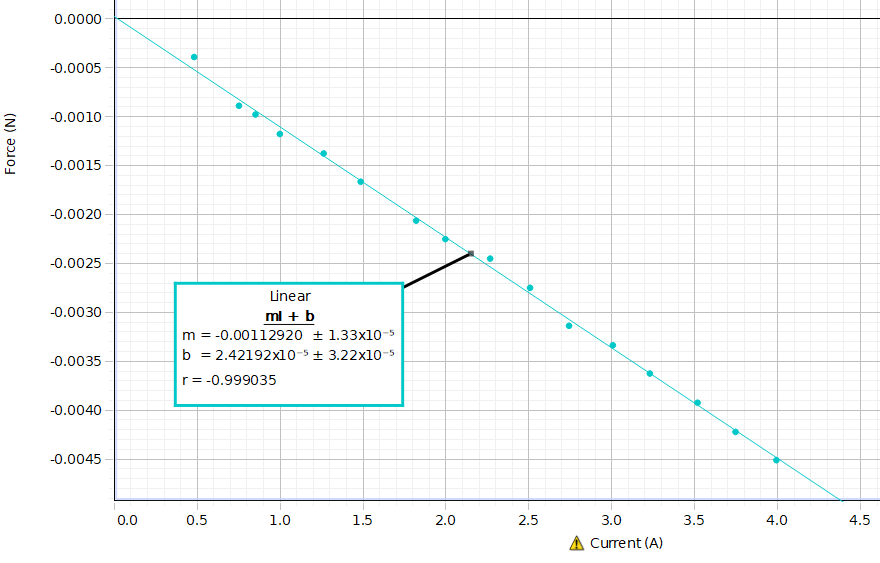
\includegraphics[width=1\textwidth]{Figures/Lab 9 set2.PNG} % Include the figure
	\caption{Part B.1: Force(N) vs Current(A)}
\end{figure}
\begin{figure}[H] % [H] forces the figure to be placed exactly where it appears in the text
	\centering % Horizontally center the figure
	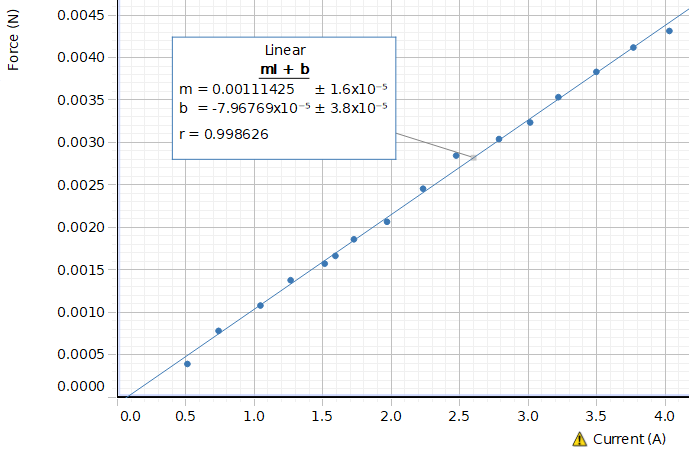
\includegraphics[width=1\textwidth]{Figures/Lab 9 set4.PNG} % Include the figure
	\caption{Part B.2: Force(N) vs Current(A)}
\end{figure}
\begin{figure}[H] % [H] forces the figure to be placed exactly where it appears in the text
	\centering % Horizontally center the figure
	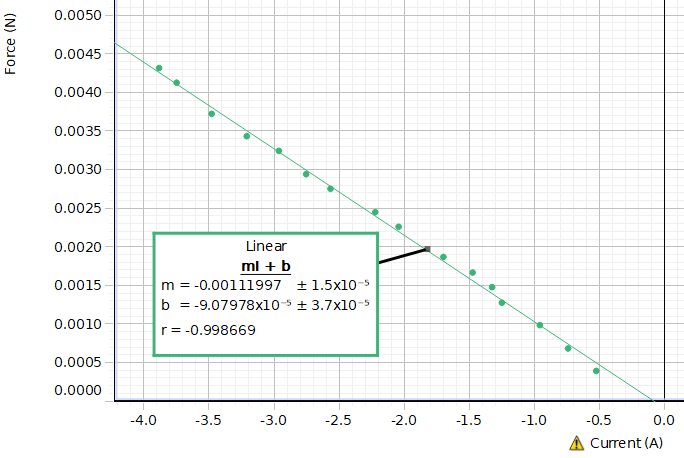
\includegraphics[width=1\textwidth]{Figures/Lab 9 set5.PNG} % Include the figure
	\caption{Part B.3: Force(N) vs Current(A)}
\end{figure}
\begin{figure}[H] % [H] forces the figure to be placed exactly where it appears in the text
	\centering % Horizontally center the figure
	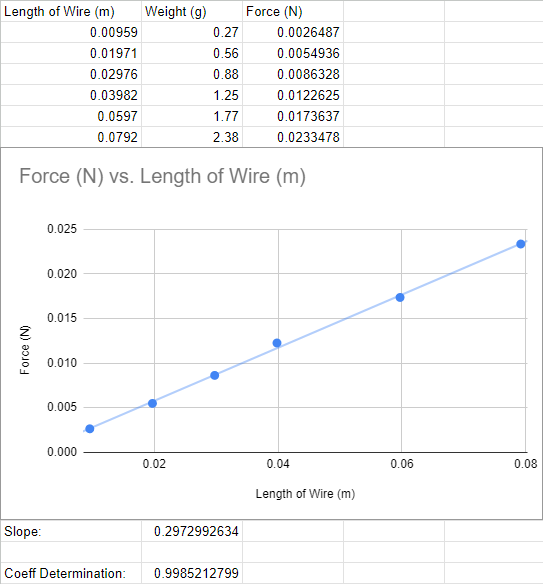
\includegraphics[width=1\textwidth]{Figures/Part C Linear Fit.png} % Include the figure
	\caption{Part C: Force(N) vs Wire Length(m)}
\end{figure}

\end{document}